\graphicspath{ {res/img/} }

\subsection{Accessibilità}
%TODO
%MEMO: per i problemi e le soluzioni addottate per l'accessibilita' vedere:
%https://github.com/Hexamini/PassioneKaraoke/issues?utf8=%E2%9C%93&q=is%3Aissue+milestone%3AAccessibilit%C3%A0+
Il sito è stato utilizzato sviluppando solamente codice XHTML 1.0 Strict, per assicurare la massima compatibilità. Per i fogli di stile è invece stato deciso di applicare CSS 3.0, per potersi avvantaggiare di nuove tecnologie grafiche e ridurre al minimo l'utilizzo di JavaScript, che invece è stato applicato per i controlli sul form di login e sulla gestione del contenuto del sito, avendo comunque una buona degradazione in caso questa tecnologia non sia disponibile nel dispositivo in uso.

\subsubsection{Colori del sito}
%TODO
I colori del sito sono stati scelti dopo diversi tentativi tramite l'utilizzo di \url{http://vischeck.com/}. Inizialmente si era stati propensi per un colore caldo, tendente al rosso/arancione, ma effettuando i test si è ottenuto i seguenti risultati:

\begin{itemize}

    \item[]
        \begin{figure}[H]

            \centering
            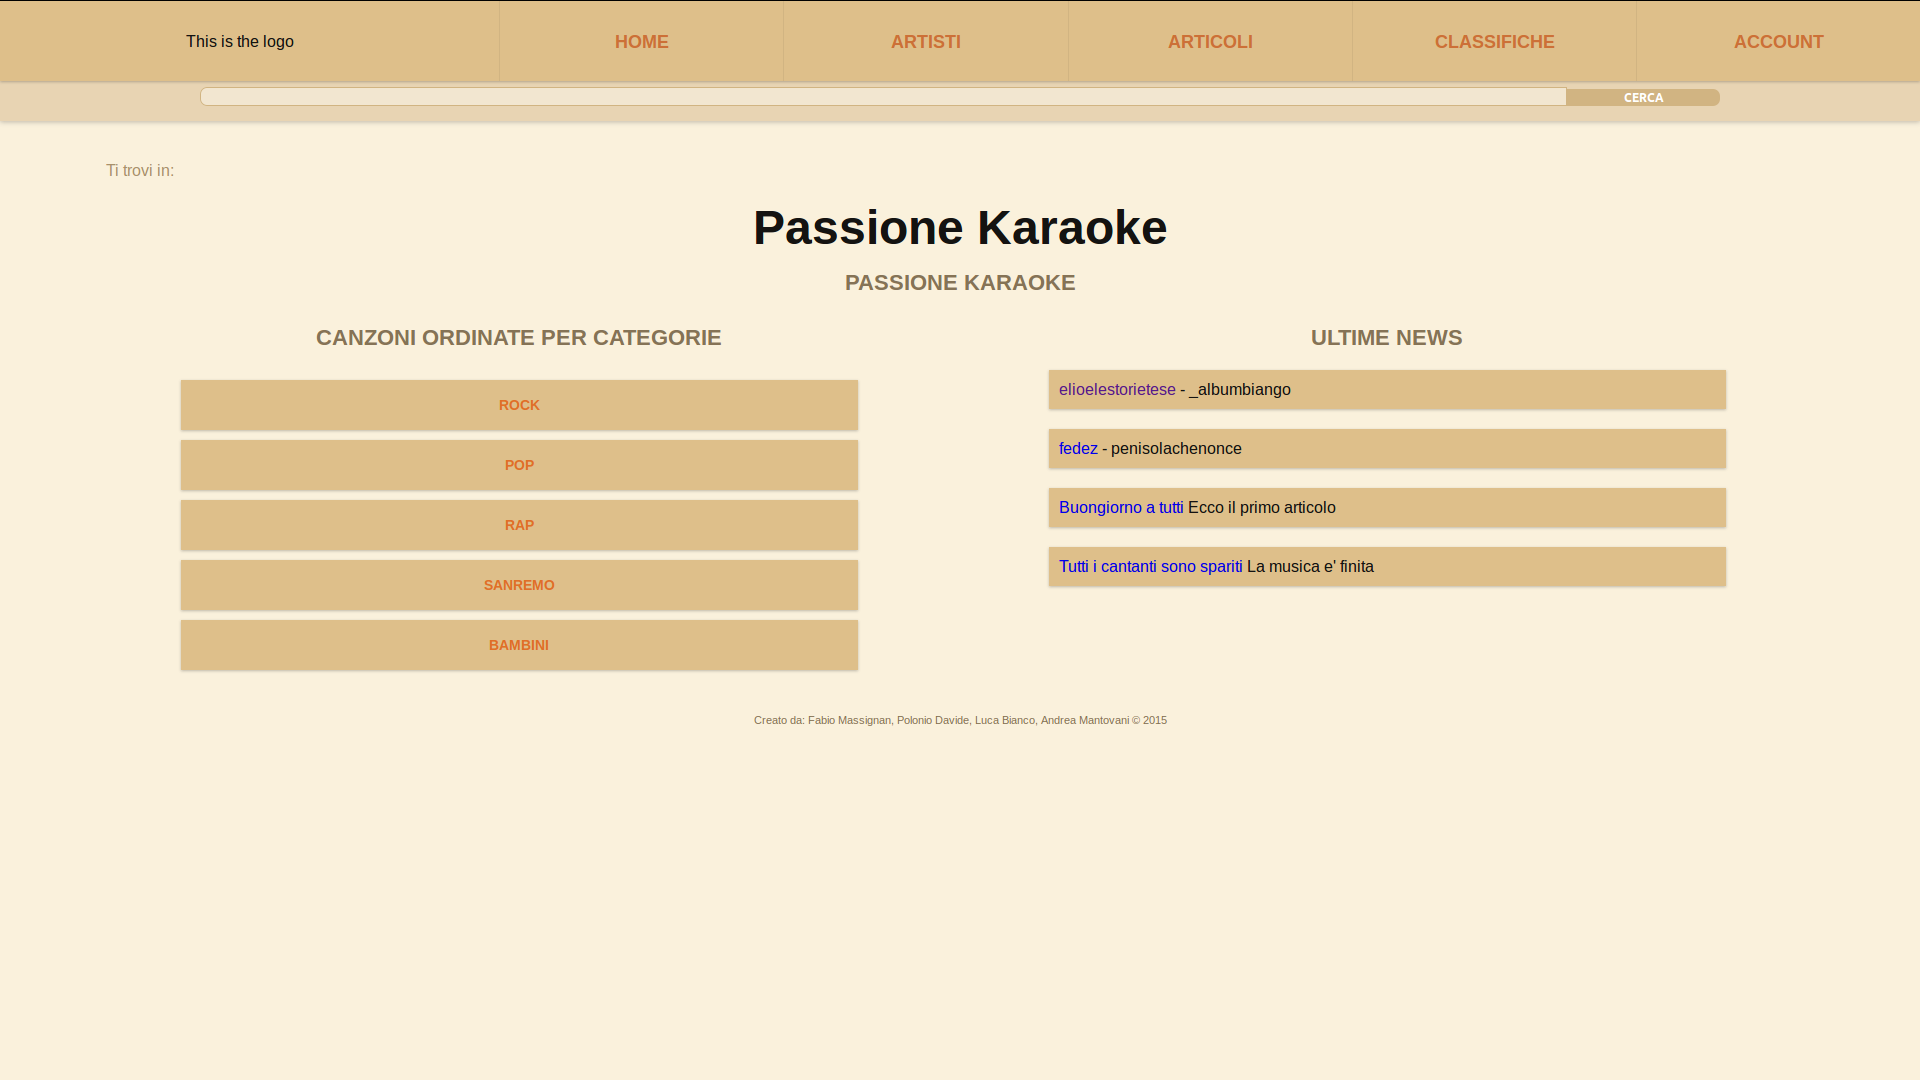
\includegraphics[scale=0.1]{firstImgNormal}
            \caption{Design del sito con vecchi colori}
        \end{figure}

    \item[]
        \begin{figure}[H]

            \centering
            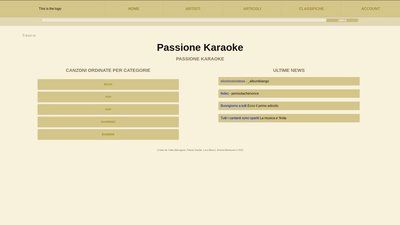
\includegraphics[scale=0.5]{firstImgDeuteranope}
            \caption{Risultati del test per \textit{Deuteranope}}
        \end{figure}

    \item[]
        \begin{figure}[H]

            \centering
            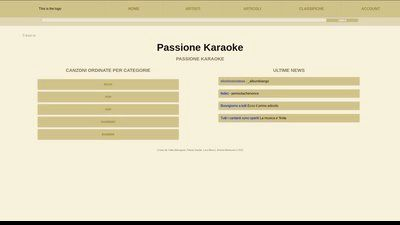
\includegraphics[scale=0.5]{firstImgProtanope}
            \caption{Risultati del test per \textit{Protanope}}
        \end{figure}

    \item[]
        \begin{figure}[H]

            \centering
            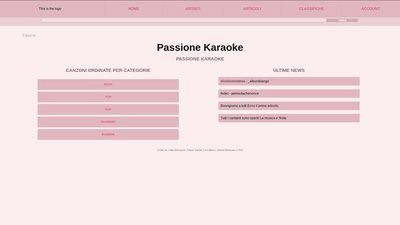
\includegraphics[scale=0.5]{firstImgTritanope}
            \caption{Risultati del test per \textit{Tritanope}}
        \end{figure}

\end{itemize}

Come si può ben vedere, i colori non ``degradano'' in maniera elegante, causando una distorsione troppo forte. Si è quindi deciso di cambiarli, ottenendo i seguenti risultati:
\begin{itemize}

    \item[]
       \begin{figure}[H]

            \centering
            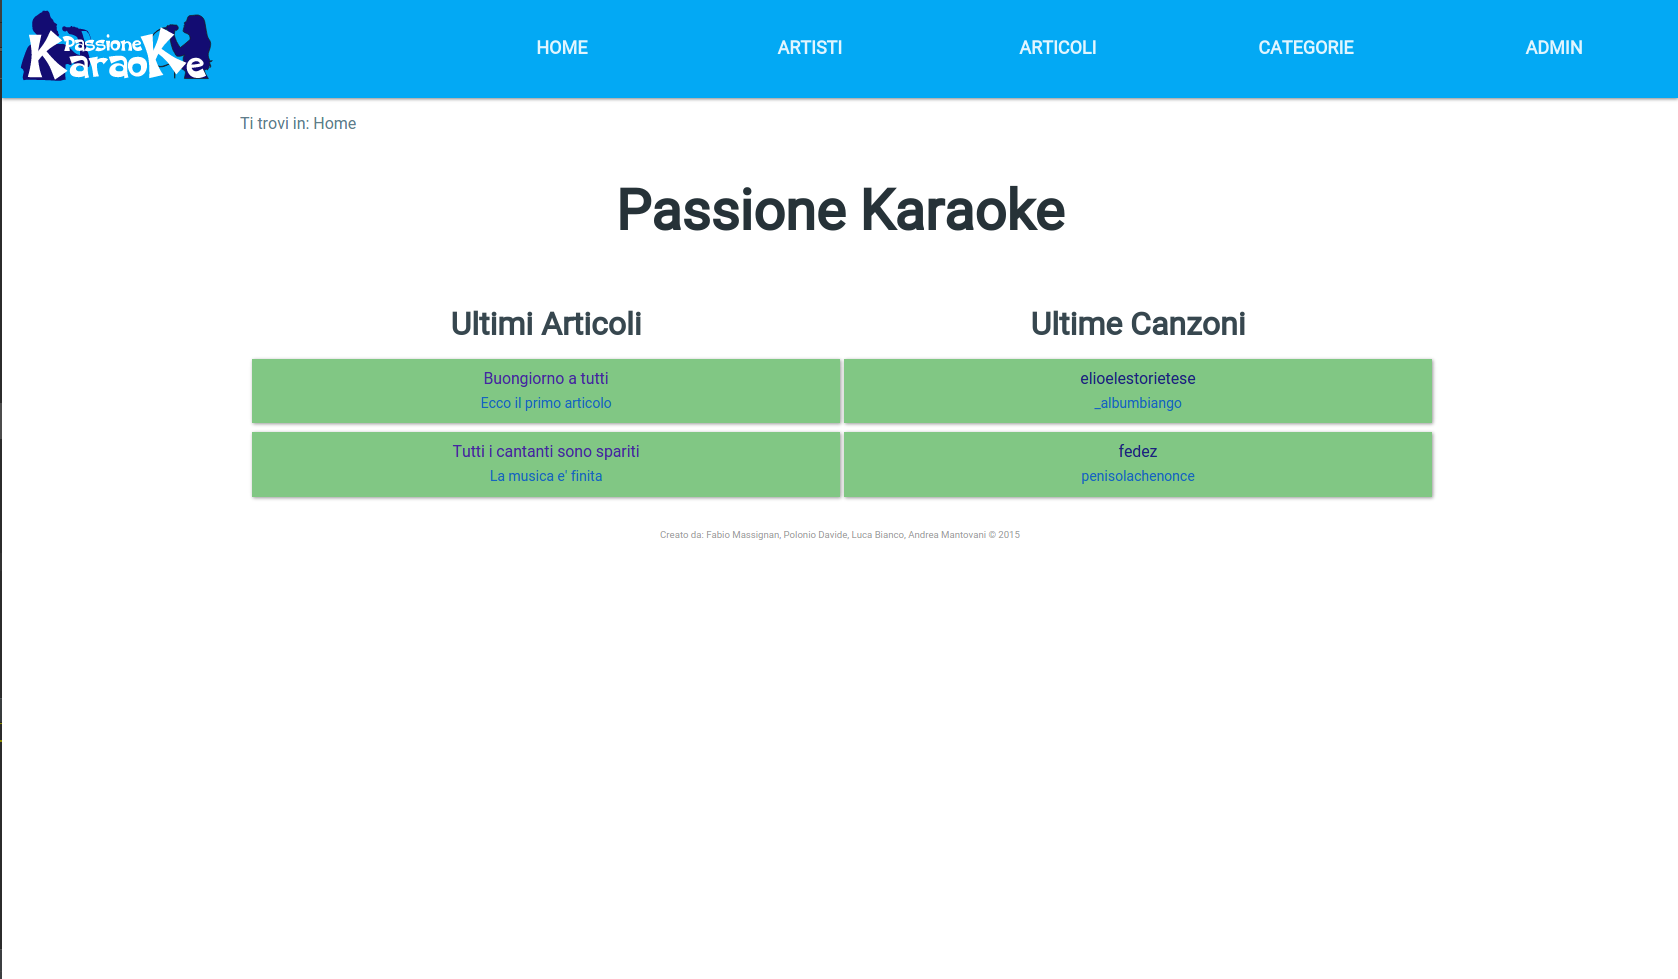
\includegraphics[scale=0.125]{lastImgNormal}
            \caption{Design del sito con i colori finali}
        \end{figure}

    \item[]
        \begin{figure}[H]

            \centering
            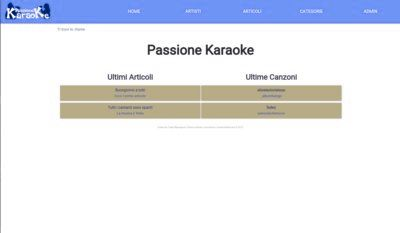
\includegraphics[scale=0.5]{lastImgDeuteranope}
            \caption{Risultati del test per \textit{Deuteranope}}
        \end{figure}

    \item[]
        \begin{figure}[H]

            \centering
            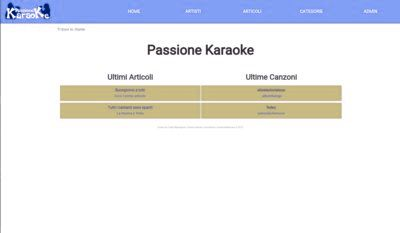
\includegraphics[scale=0.5]{lastImgProtanope}
            \caption{Risultati del test per \textit{Protanope}}
        \end{figure}

    \item[]
        \begin{figure}[H]

            \centering
            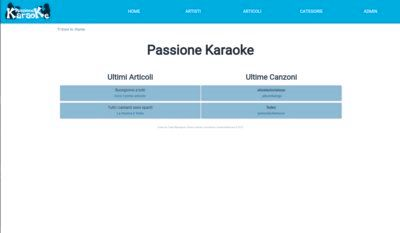
\includegraphics[scale=0.5]{lastImgTritanope}
            \caption{Risultati del test per \textit{Tritanope}}
        \end{figure}

\end{itemize}

Il resto del sito si basa su questa gamma di colori. \`E stata presa l'homepage come esempio principale.

\subsubsection{Colori dei bottoni per esprimere preferenze}
Per accertarsi di avere una accessibilit\`a dal punto di vista visivo completa, si \`e proceduto a controllare anche i bottoni per esprimere la preferenza o meno di una canzone: questa operazione di controllo in particolare \`e stata effettuata in quanto non rappresentano convenzioni standard, ma essendo convenzioni interne del sito si \`e preferito assicurarsi che tutti gli utenti con capacit\`a visive siano in grado di comprendere appieno il messaggio trasmesso tramite queste icone.

\begin{figure}[H]
    \centering
    \begin{subfigure}[b]{0.4\textwidth}
        
\includegraphics[scale=0.5]{microphoneLike}
        \caption{Icona usata per esprimere un apprezzamento positivo}
    \end{subfigure}
    ~
    \begin{subfigure}[b]{0.4\textwidth}
        
\includegraphics[scale=0.5]{microphoneNotLike}
        \caption{Icona usata per esprimere un apprezzamento negativo}
    \end{subfigure}
    ~
    \caption{Icone usate per esprimere preferenze all'interno del sito}
\end{figure}

\`E importante far notare come sia stato scelto il blu al posto di un pi\`u comune verde: dopo un test effettuato tramite \url{http://www.vischeck.com/} si \`e notato che non era abbastanza accessibile, e che non era presente una distinzione abbastanza forte tra i colori delle due icone. Dopo aver cambiato il colore di una delle due icone sono stati ri-effettuati i test, ottenendo i seguenti risultati:
\begin{itemize}

    \item[]

        \begin{figure}[H]
            \centering
            \begin{subfigure}[b]{0.3\textwidth}
                
\includegraphics[scale=0.3]{microphoneLikeDeuteranope}
                \caption{Risultati del test per \textit{Deuteranope}}
            \end{subfigure}
        ~
            \begin{subfigure}[b]{0.3\textwidth}
                
\includegraphics[scale=0.3]{microphoneLikeProtanope}
                \caption{Risultati del test per \textit{Protanope}}
            \end{subfigure}
        ~
            \begin{subfigure}[b]{0.3\textwidth}
                
\includegraphics[scale=0.3]{microphoneLikeTritanope}
                \caption{Risultati del test per \textit{Tritanope}}
            \end{subfigure}
        ~
            \caption{Risultati del test per il bottone per esprimere una preferenza positiva}
        \end{figure}

    \item[]
    \begin{itemize}

        \begin{figure}[H]
            \centering
            \begin{subfigure}[b]{0.3\textwidth}
                
\includegraphics[scale=0.3]{microphoneNotLikeDeuteranope}
                \caption{Risultati del test per \textit{Deuteranope}}
            \end{subfigure}
        ~
            \begin{subfigure}[b]{0.3\textwidth}
                
\includegraphics[scale=0.3]{microphoneNotLikeProtanope}
                \caption{Risultati del test per \textit{Protanope}}
            \end{subfigure}
        ~
            \begin{subfigure}[b]{0.3\textwidth}
                
\includegraphics[scale=0.3]{microphoneNotLikeTritanope}
                \caption{Risultati del test per \textit{Tritanope}}
            \end{subfigure}
        ~
            \caption{Risultati del test per il bottone per esprimere una preferenza negativa}
        \end{figure}

    \end{itemize}

\end{itemize}

\paragraph*{Contrasto e leggibilit\`a}
\`E stato considerato importante anche considerare la leggibilit\`a del testo per quelle persone che riportano problemi visivi. Un test sul contrasto tra testo e sfondo \`e stato effettuato utilizzando il tool reperibile al seguente indirizzo: \url{http://leaverou.github.io/contrast-ratio/#\%23E1F5FE-on-\%2301579B}.
I risultati ottenuti sono stati i seguenti: %TODO: da elencare i risultati ottenuti!

\subsubsection{Form e segnalazione errori}
\label{form-accessibilita}
Nel sito è possibile, da parte dell'utente, l'inserimento di dati tramite l'utilizzo di form (per esempio per eseguire un login). È stato quindi necessario rendere i form accessibili tramite diversi accorgimenti: %elencare quali
Sono state effettuate anche delle scelte di usabilità, esplicate in \ref{form-usabilita}
